% Document information
\newcommand{\titleinfo}{Zusammenfassung ComEng1}
\newcommand{\authorinfo}{Sandro Pedrett}
\newcommand{\version}{0.1}
\newcommand{\versioninfo}{FS21}
% Header
\include{Template/Header}

% Setup Source Code
\lstset{ 
	backgroundcolor=\color{white},   % choose the background color; you must add \usepackage{color} or \usepackage{xcolor}; should come as last argument
	basicstyle=\footnotesize,        % the size of the fonts that are used for the code
	breakatwhitespace=false,         % sets if automatic breaks should only happen at whitespace
	breaklines=true,                 % sets automatic line breaking
	captionpos=b,                    % sets the caption-position to bottom
	commentstyle=\color{ForestGreen},    % comment style
	escapeinside={\%*}{*)},          % if you want to add LaTeX within your code
	extendedchars=true,              % lets you use non-ASCII characters; for 8-bits encodings only, does not work with UTF-8
	frame=single,	                   % adds a frame around the code
	keepspaces=true,                 % keeps spaces in text, useful for keeping indentation of code (possibly needs columns=flexible)
	language=C,                 % the language of the code
	numbersep=5pt,                   % how far the line-numbers are from the code
	rulecolor=\color{black},         % if not set, the frame-color may be changed on line-breaks within not-black text (e.g. comments (green here))
	showspaces=false,                % show spaces everywhere adding particular underscores; it overrides 'showstringspaces'
	showstringspaces=false,          % underline spaces within strings only
	showtabs=false,                  % show tabs within strings adding particular underscores
	stepnumber=2,                    % the step between two line-numbers. If it's 1, each line will be numbered
	tabsize=2,	                   % sets default tabsize to 2 spaces
	title=\lstname                   % show the filename of files included with \lstinputlisting; also try caption instead of title
}
% Document
\begin{document}

\section{Einführung}
TODO


\section{Embedded Systems}
Keywords: Mikroprozessortechnik, Mikroprozessor, Mikroarchitektur

\begin{itemize}[nosep]
	\item Echtzeitfühigkeit
	\item Zuverlässigkeit
	\item Informationssicherheit
	\item Ressourcen	
	\item Kostendruck	
\end{itemize}
~\\
DSP: in audio, video, AI etc
\\
SoC: ASIC, FPGA, Soft-Core

\subsection{Bestandteile}
\begin{itemize}[nosep]
	\item CPU
	\item Speicher (RAM, ROM)
	\item I/O Einheiten
	\item Systembus $\rightarrow$ Master-Slave-Prinzip
	\item IRQ Fähigkeit
	\item Timer, OZI
\end{itemize}

\subsubsection{Architektur}
\subsection{Architektur}
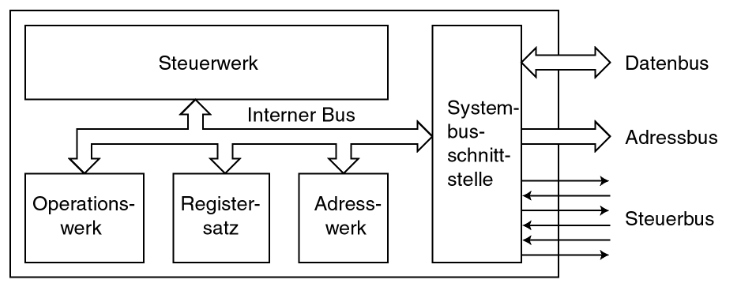
\includegraphics[width=\columnwidth]{Images/Blockschema}
Der \textbf{Registersatz} enthält einen Satz von Registern,  mit dem Daten innerhalb des Prozessors  gespeichert  werden  können.   Ein  Register  ist  eine  Gruppe  vonFlipflops mit gemeinsamer Steuerung.\\
Das \textbf{Operationswerkführt}  die  eigentliche  Verarbeitung,  d.h.   die  logischen  und arithmetischen Operationen, an den übergebenen Daten aus.\\
Das \textbf{Steuerwerk ist} verantwortlich für die Ablaufsteuerung sowohl im Inneren des Prozessors als auch im restlichen System.\\
Das \textbf{Adresswerk} erzeugt die erforderlichen Adressen, um auf Daten und Code im Hauptspeicher zugreifen zu können.\\
Die \textbf{Systembus-Schnittstelle} enthält Puffer- und Treiberschaltungen, um den Datenverkehr über den Systembus abzuwickeln.

~\\
\begin{itemize}[nosep]
	\item Neumann vs Havard
		\begin{itemize}[nosep]
			\item Von-Neumann $\rightarrow$ Gleicher Systembus, Bottleneck!
			\item Havard $\rightarrow$ ein Bus für Daten, einer für Programm!
		\end{itemize}
	\item Mikroprozessor vs Mikrocontroller (RAM)
\end{itemize}

\begin{itemize}[nosep]
	\item CISC vs RISC
	\begin{itemize}[nosep]
		\item CISC besitzen viele spezialisierte Instruktionen.
		\item RISC besitzen wenige dafür einfache Instruktionen.
	\end{itemize}
\end{itemize}

\subsection{Polling/IRQ}
\todo{Woche 03}
\section{Informationsdarstellung}
\subsection{Begriffe}
\todo{Woche2: Word abhängig von Verarbeitungsbreite.}

\subsection{Signale}
\todo{Woche2: Signale, Daten-Meldungen, Datenströme}

\subsection{Zahlendarstellung}
\todo{TODO}
\subsubsection{Vorzeichenlose Ganzzahl}
\[W = \sum_{i=0}^{n-1}d_i\cdot 2^i\]
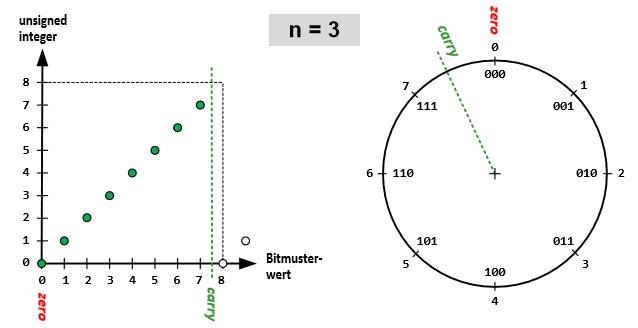
\includegraphics[width=\linewidth]{Images/ganzzahl}


\subsubsection{Signed Magnitued}
\[W = (-1)^{n-1} \cdot \sum_{i=0}^{n-1}d_i\cdot 2^i\]
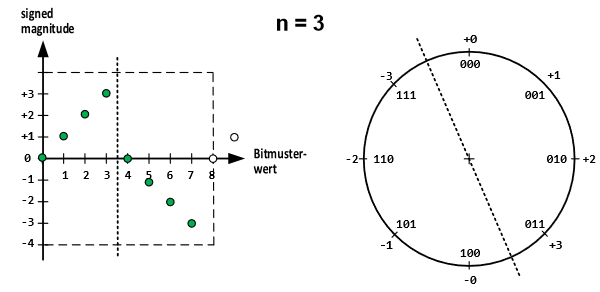
\includegraphics[width=\linewidth]{Images/signedmagnetude}

\subsubsection{Einerkomplement}
\[
W =
\begin{cases}
	\sum_{i=0}^{n-2}d_i \cdot 2^i & d_{n-1} > 0 \\
	\left(\sum_{i=0}^{n-2}d_i \cdot 2^i\right) - \sum_{i=0}^{n-2}2^i & d_{n-1} < 0 
\end{cases}
\]
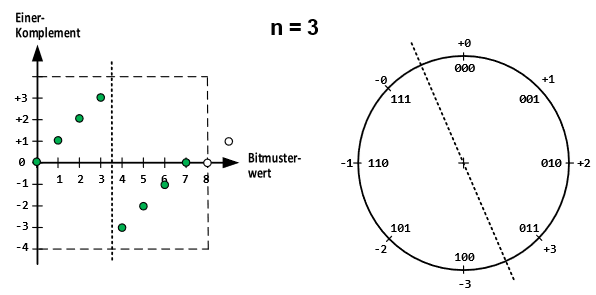
\includegraphics[width=\linewidth]{Images/einerkomplement}


\subsubsection{Zweierkomplement}
\[W = \left(\sum_{i=0}^{n-1}d_i\cdot 2^i\right) - (d^{n-1}\cdot2^n)\]
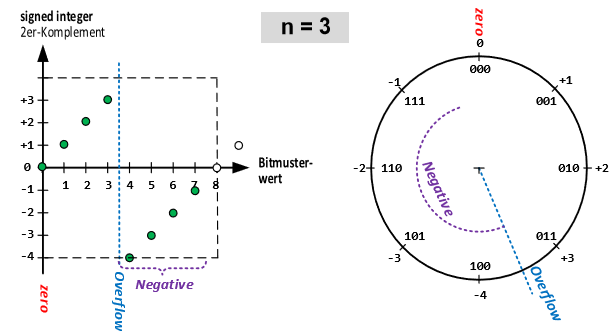
\includegraphics[width=\linewidth]{Images/zweierkomplement}

\subsubsection{Excess-Code (EX)}
\[W = \left(\sum_{i=0}^{n-1}d_i\cdot 2^i\right) - (2^{n-1})\]
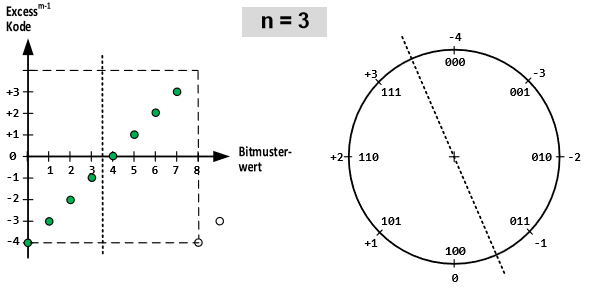
\includegraphics[width=\linewidth]{Images/ex}


\subsubsection{Festkommazahl}
\todo{Basisformat, Fraktionale Zahlen, IQ-Zahlen}

\subsubsection{Gleitkommazahl}
Binär zu Dezimal IEEE 754\\
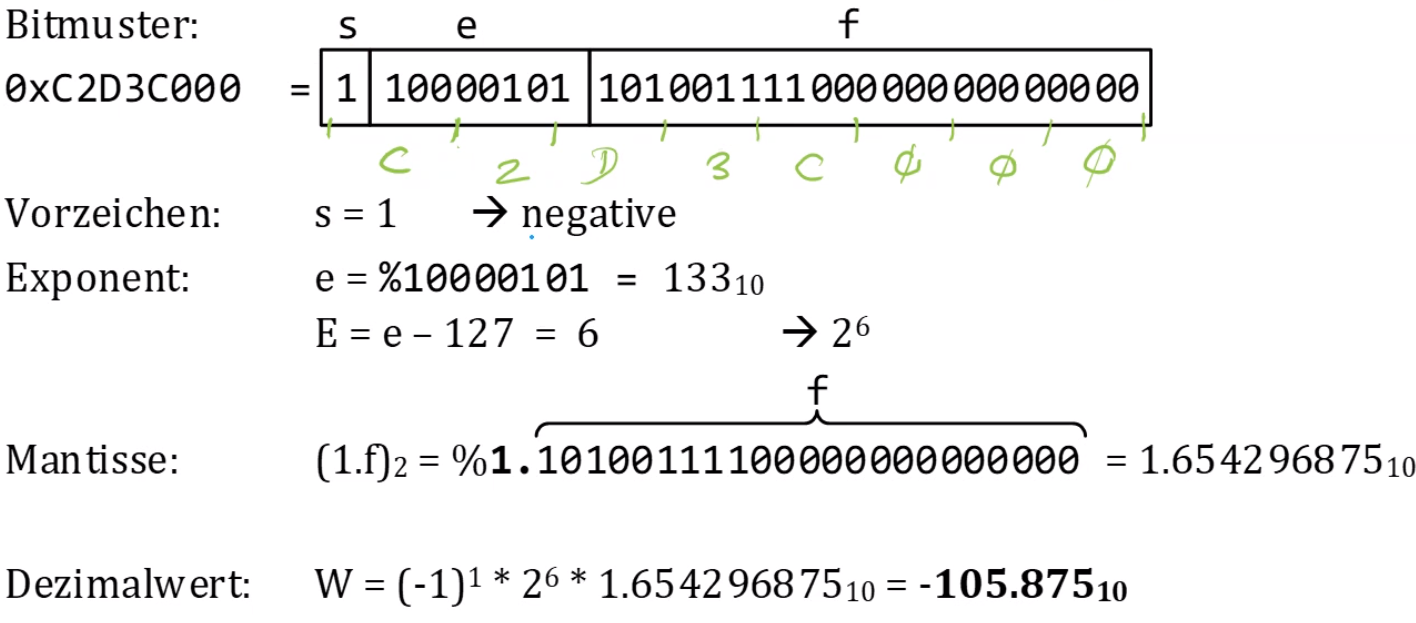
\includegraphics[width=\linewidth]{Images/float}

\subsubsection{BCD-Code}
\input{Sections/Zahlen und Zeichencodes}
\section{PicoBlazer}
\subsection{Flags}
\begin{enumerate}[nosep]
	\item Zero Z
	\item Carry C
	\item Overflow V
	\item Negative N
\end{enumerate}


\subsection{Addressbereiche}
\todo{Zeige Instruktionen welche in jeweilige Bereich schreiben kann.
% TODO: \usepackage{graphicx} required
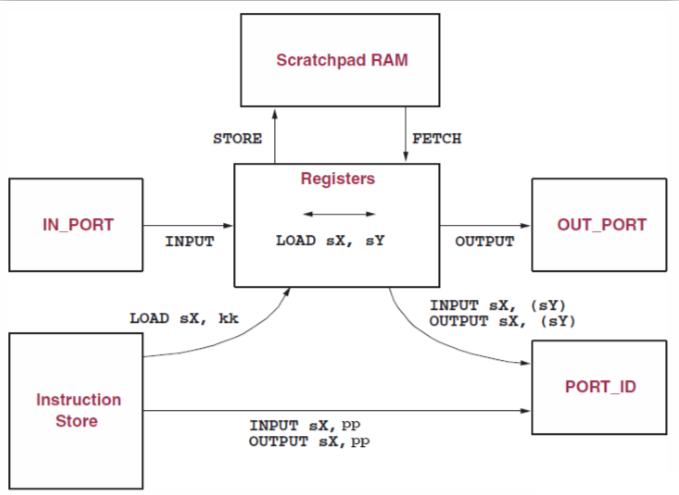
\includegraphics[width=\columnwidth]{Images/datamovement}
}
\begin{enumerate}[nosep]
	\item Instruction PROM, ProgramFlowControl
	\item General-Purpose Register, Moving Data
	\item Scratchpad RAM, Moving Data
	\item I/O Port, Moving Data
	\item CALL/RETURN Stack, ProgramFlowControl
\end{enumerate}

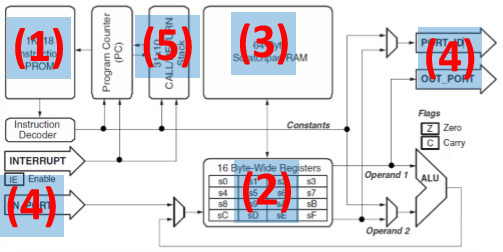
\includegraphics[width=\columnwidth]{Images/addressranges}


\subsection{Asynchrone Events}
\subsubsection{IRQ Event}
Ein IRQ-Event ist ein asynchrones Event, welches zu einer Unterbrechung des normalen Programmablaufs führen \textit{kann}. Der Ablauf in der Hardware ist wie folgt definiert:
\begin{lstlisting}
// (0) only respond to IRQ input if IE flag is set, i.e. after EINT or RETI ENABLE instruction
if ((IE = 1) and (IRQ input = HIGH)) {
	// (1) clear the IE FLAG
	IE <- 0
		
	// (2) push	the current PC to top of stack (TOS). Return Value
	TOS <- PC
		
	// (3) preseve flags
	PRESERVED_CARRAY <- CARRY
	PRESERVED_ZERO <- ZERO
		
	// (4) load PC with IRQ-Vec
	PC <- $3FF
}
\end{lstlisting}

\subsubsection{RESET Event}
Ein RESET-Event ist ein asynchrones Event, welches zu einem Neustart der CPU führt. Dies löscht die Register und ScratchPad RAM \underline{nicht}! Der Ablauf in der Hardware ist wie folgt definiert:
\begin{lstlisting}
// (0) only respond if priority is high
if (RESET input = HIGH) {
	// (1) Clear PC
	PC <- 0
	
	// (2) disable IRQ
	IE <- 0
		
	// (3) Reset flags
	CARRY <- 0
	ZERO <- 0
}
\end{lstlisting}
\section{Assembler-Code}
\subsection{If/Else}
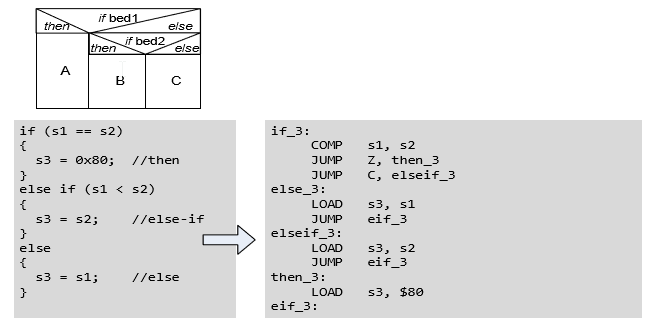
\includegraphics[width=\linewidth]{Images/ifelseif}
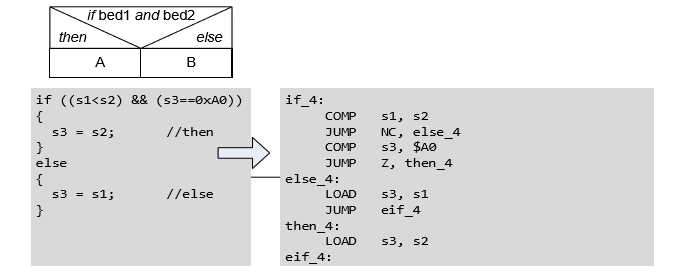
\includegraphics[width=\linewidth]{Images/ifelseif_multiple}


\subsection{Switch-Case}
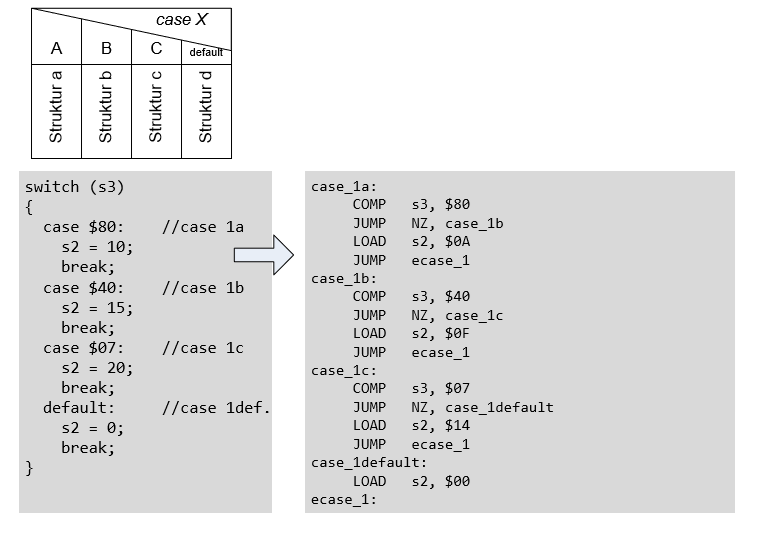
\includegraphics[width=\linewidth]{Images/switchcase}

\subsection{Loops}
Abweisende Loops prüfen vor dem Body zB While/Do oder For. Nicht abweisende Loops werden mindestens einmal durchlaufen zB while/do\\
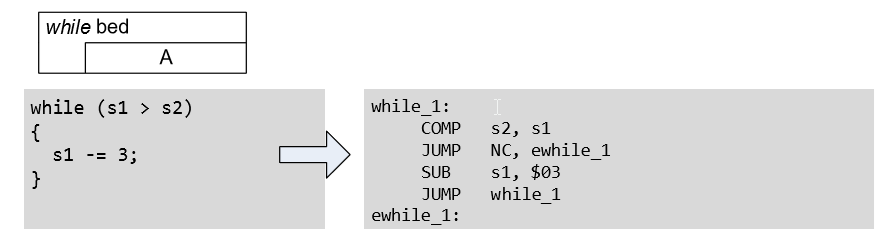
\includegraphics[width=\linewidth]{Images/while}
\newpage
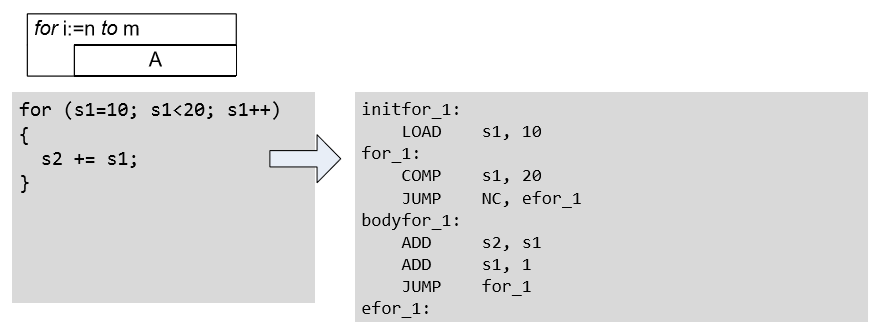
\includegraphics[width=\linewidth]{Images/for}

\subsection{Subroutine}
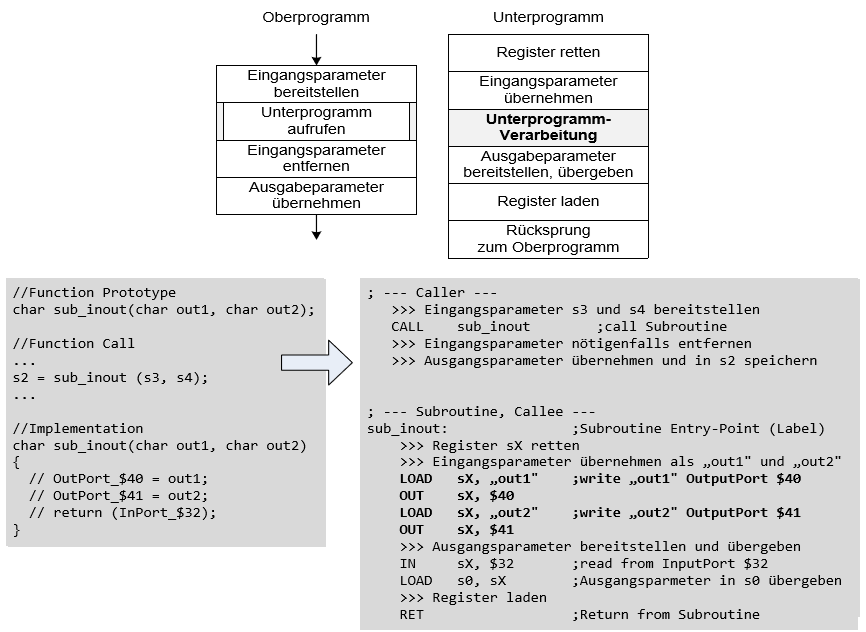
\includegraphics[width=\linewidth]{Images/subroutine}
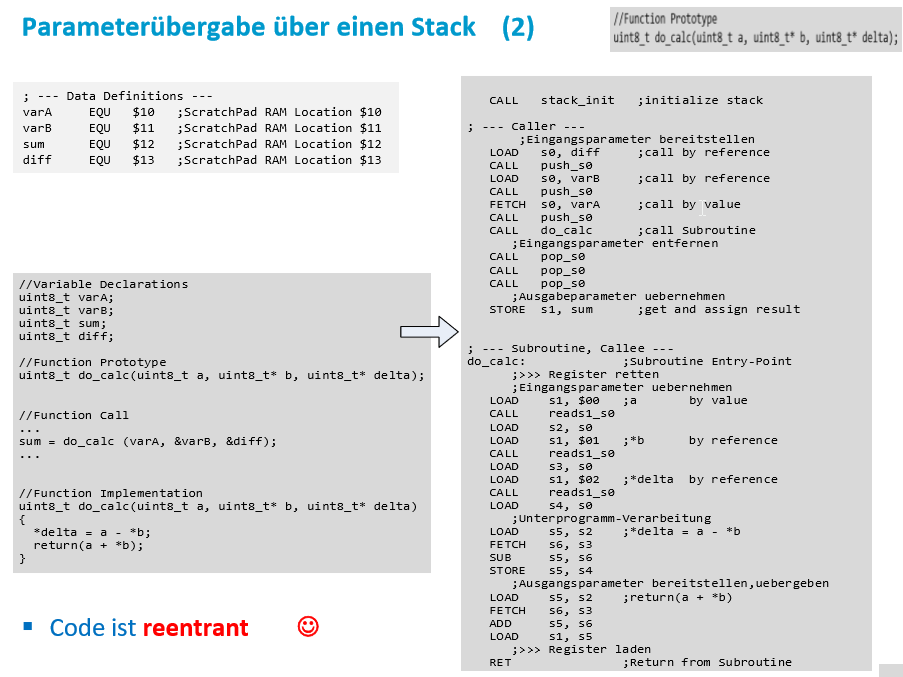
\includegraphics[width=\linewidth]{Images/subroutine_mitparam}



\end{document}